\documentclass[11pt]{article}
\usepackage{enumitem}
\usepackage{hyperref}
\hypersetup{
	colorlinks=true,
	linkcolor=blue,
	filecolor=magenta,      
	urlcolor=cyan,
}
\usepackage{graphicx}
\usepackage{amsmath}
\usepackage[utf8]{inputenc}
\usepackage{mathtools}
\usepackage[caption=false]{subfig}
\usepackage{soul}
\usepackage[top=0.75in, bottom=0.75in, left=0.75in, right=0.75in]{geometry}
\usepackage[margin=1.5cm]{caption}
\usepackage{epsfig,amsmath}
\DeclarePairedDelimiter\abs{${\lvert}$}{${\rvert}$}%
\usepackage{titlesec,color}
\usepackage{kpfonts}
\usepackage{empheq}
\usepackage{palatino}
\usepackage{graphicx,wrapfig}
\setlength{\parskip}{1em}
\setlength{\parindent}{0pt}
\usepackage{array}
\usepackage{gensymb}
\usepackage{soul}
\usepackage{grffile}
\usepackage{multicol}
\usepackage{listings}
\usepackage{color}
\usepackage{tcolorbox}
\usepackage{courier}
\usepackage[T1]{fontenc}
\usepackage{arial}
\usepackage{multicol}
\setlength\columnsep{0.3in}
\tcbuselibrary{listings,skins}
\tolerance=1
\emergencystretch=\maxdimen
\hyphenpenalty=10000
\hbadness=1000

\definecolor{dkgreen}{rgb}{0,0.6,0}
\definecolor{gray}{rgb}{0.5,0.5,0.5}
\definecolor{mauve}{rgb}{0.58,0,0.82}

\begin{document}
	
\renewcommand*\rmdefault{phv}
\fontfamily{phv}\selectfont

\newcommand{\avg}[1]{\left<{#1}\right>}
\newcommand{\hence}{\hspace{1cm}\Longrightarrow\hspace{1cm}}
\renewcommand{\ni}{\noindent}
\newcommand{\din}{\indent \indent}
\newcommand{\mni}{\medskip \noindent}
\newcommand{\bni}{\bigskip \noindent}
\newcommand{\sni}{\smallskip \noindent}
\newcommand{\pr}{{\rm Prob}}
\newcommand{\mon}{\begin{displaymath}}
\newcommand{\moff}{\end{displaymath}}
\newcommand{\sumi}[1]{\sum_{{#1}=-\infty}^{\infty}}
\renewcommand{\b}[1]{\mbox{\boldmath ${#1}$}}
\newcommand{\sumy}{\sum_{\b{y}}}
\newcommand{\sumz}{\sum_{\b{z}}}
\newcommand{\pd}[2]{\frac{\partial {#1}}{\partial {#2}}}
\newcommand{\od}[2]{\frac{d {#1}}{d {#2}}}
\newcommand{\odat}[3]{\left. \frac{d {#1}}{d {#2}} \right|_{#3}}
\newcommand{\inti}{\int_{-\infty}^{\infty}}
\newcommand{\eon}{\begin{equation}}
\newcommand{\eoff}{\end{equation}}
\newcommand{\eaon}{\begin{eqnarray}}
\newcommand{\eaoff}{\end{eqnarray}}
\newcommand{\e}[1]{\times 10^{#1}}
\newcommand{\chem}[2]{{}^{#2} \mathrm{#1}}
\renewcommand{\sb}{s}
\newcommand{\s}{s}
\newcommand{\zetaexp}{\left( \zeta e^{q \s t} \right)}
\newcommand{\taunuc}{\tau_{nuc}}
\newcommand{\eq}[1]{Eq. (\ref{#1})}\
\newcommand{\ev}[1]{\langle #1 \rangle}
\newcommand*\mean[1]{${\bar{#1}}$}
\newcolumntype{L}{>{\centering\arraybackslash}m{5cm}}


\begin{center}
\Large CS109 Group 10 - Scope of Work
\end{center}
\begin{center}
\small Guilherme Braz, James May, Shristi Pandey, Zach Werkhoven
\end{center}

\textbf{Group Number:} \quad 10\newline

\textbf{Have you met/communicated with your fellow teammates?}

We have met twice as a group via video conference and have setup a slack team to handle our day-to-day communication.
\vspace*{0.3cm}

\textbf{Have you met/communicated with your assigned TF?}

We have been in contact with our TF (Justin Lee) by email and held a video conference with him over the weekend.
\vspace*{0.3cm}

\textbf{Has your team formulated a well-defined question to address in your project, based on the project description and references?}

We have defined an intermediate goal of conducting exploratory data analysis to identify features from that ADNI database that will allow us to develop a model for predicting patient prognosis. Our goal will become more well-defined once we have conducted additional research and have a better grasp on the structure and availability of the many possible features in the data set. An important step toward this goal will be defining our response variable. Potential response variables include categorical features such as diagnosis (DXSUM or DXCHANGE) or continuous features such as the Alzheimer's Disease Assessment Score (ADAS). We will focus on these response variable candidates in greater detail during preliminary EDA.
\vspace*{0.3cm}

\textbf{Briefly describe your team’s plans for work to be completed by Nov 28 (milestone three). Please assign specific tasks to team members and deadlines for when these tasks are to be completed.}

Please see the below (Table 1) for a detailed description of our tentative work plan.

\begin{center}
\begin{figure}[t!]
	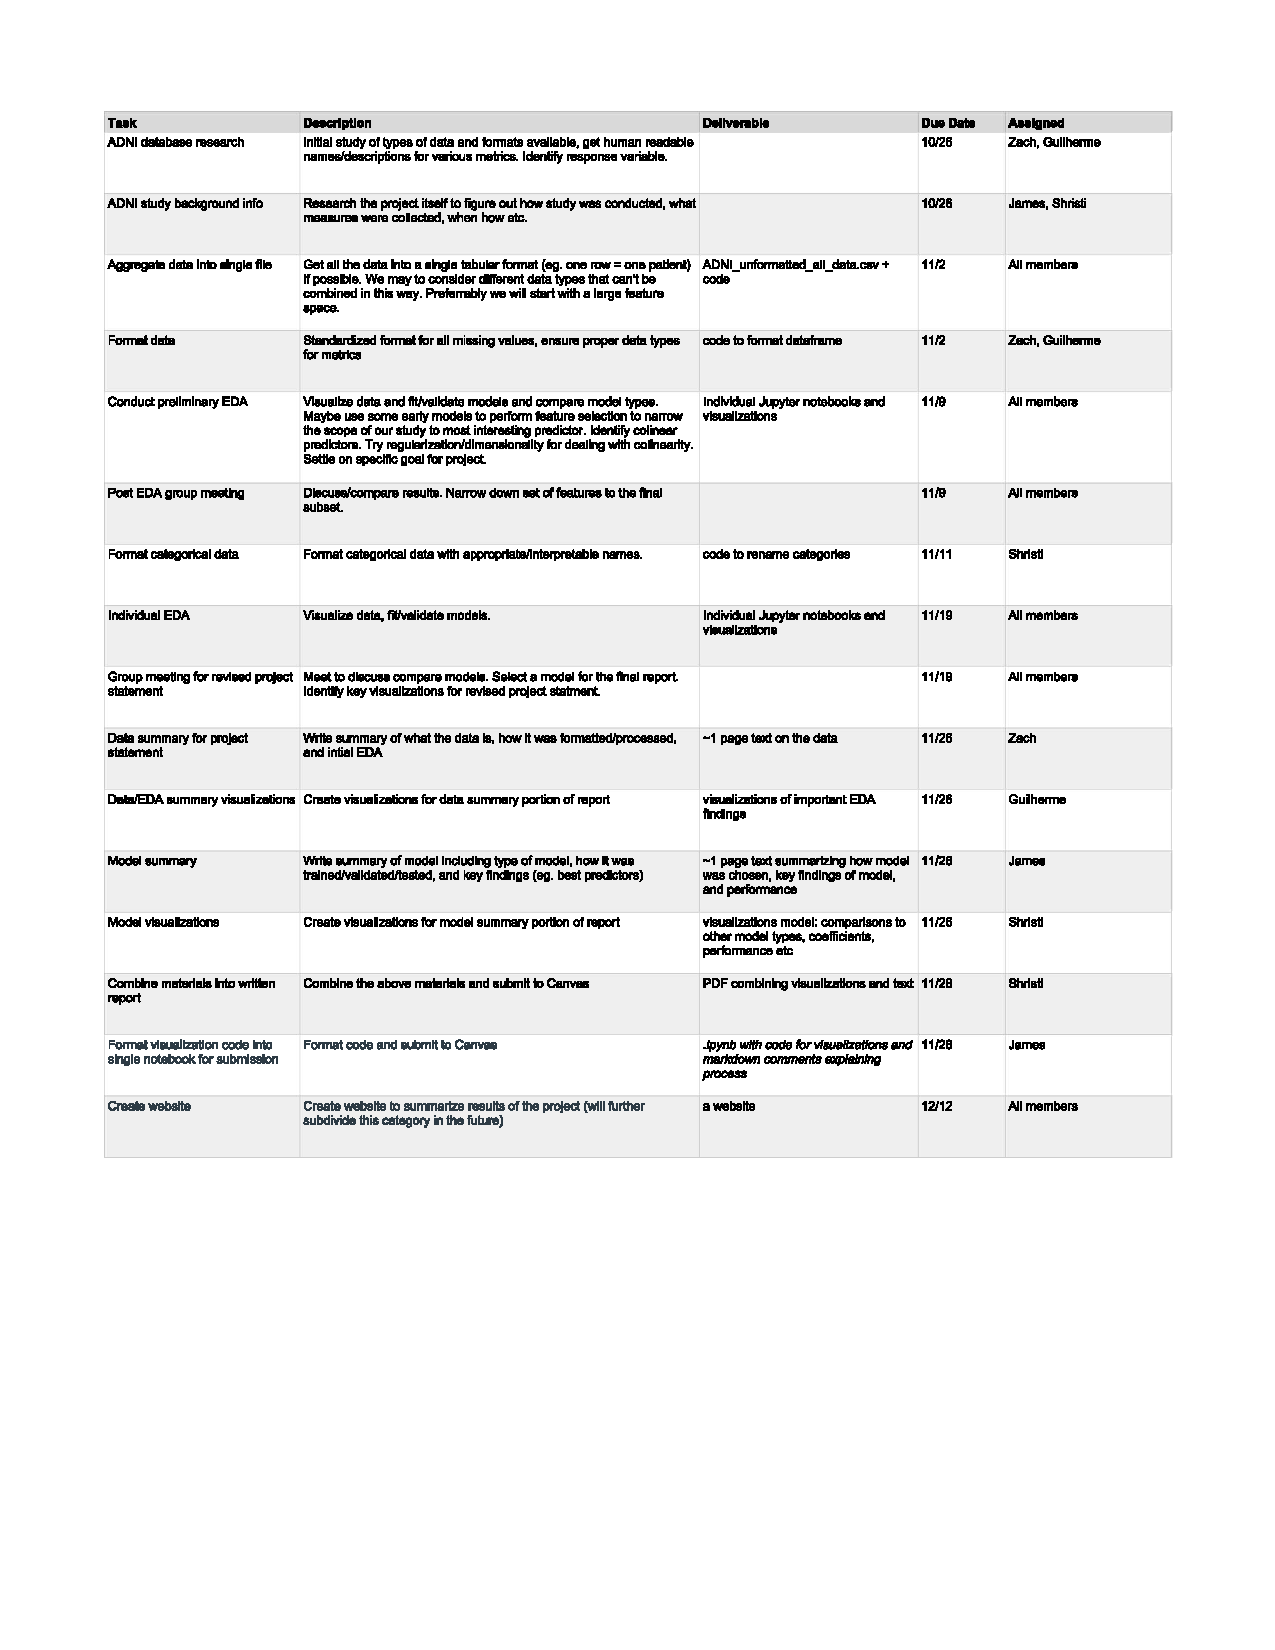
\includegraphics[width=0.95\textwidth]{schedule.pdf}
	\vspace*{-6.5cm}
	\caption*{\footnotesize Table 1 - Tentative description of tasks, due dates, and division of labor for Group 10 final project}
\end{figure}
\end{center}

\end{document}